\section{Experience}
\label{sec:experience}

To evaluate \DSU, we used it to update three open-source servers written
in Java: the Jetty webserver\footnote{\url{http://www.mortbay.org}},
JavaEmailServer,\footnote{\url{http://www.ericdaugherty.com/java/mailserver/}}
an SMTP and POP e-mail server, and CrossFTP server.\footnote{\url{http://www.crossftp.com/}}
These programs belong to a class that
should benefit from DSU because they typically run continuously. DSU
would enable deployments to incorporate bug fixes or add new features
without having to halt currently-running sessions.  

We explored
updates corresponding to releases made over roughly one to two years
of each program's lifetime.  Of the 22 updates we considered, \DSU{} could
support 20 of them---the two updates we could not apply changed
classes with infinitely-running methods, and thus no safe point could
be reached.  To our knowledge, no existing DSU system
for Java could support all these updates; indeed, previous systems
with simple support for updating method bodies would be able to handle only 9 of the 22 updates.  Although \DSU{} cannot support every
update, it is the first DSU system for Java
that has been shown to support changes to realistic programs as they
occur in practice over a long period of time.

In the rest of this section, we first examine the performance impact of
\DSU{}, and then look at updates to each of the three applications in
detail.

\begin{figure}[t]
\begin{small}
\begin{center}
\begin{tabular}{|l|c|c|c|c|} \hline \T
Config.                & \multicolumn{2}{c|}{Throughput (MB/s)}  & \multicolumn{2}{c|}{Latency (ms)} \\ \cline{2-5}
                       & Median   & Quartiles \T                 & Median & Quartiles                \\ \hline \T
\JikesRVM{}            & 122.437  & 121.44--123.32               & 0.442  & 0.394--0.496             \\
\DSU{}                 & 121.308  & 121.12--121.41               & 0.349  & 0.341--0.351             \\
\DSU{} upd             & 121.242  & 121.09--121.29               & 0.345  & 0.341--0.349             \\ \hline
\end{tabular}
\end{center}
\end{small}
% \caption{Throughput and latency measurements for Jetty webserver v5.1.6
% showing median and semi-interquartile range\label{tab:jetty}}
\begin{center}
\scalebox{0.63}{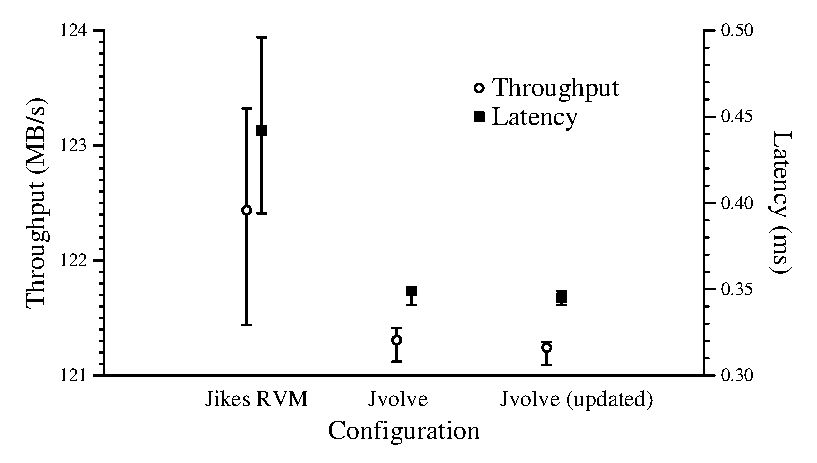
\includegraphics{graphs/jetty-throughput-latency}}
\caption{Throughput and latency measurements of Jetty webserver v5.1.6\label{fig:jetty}}
\end{center}
\end{figure}

\begin{table*}[t]
\begin{footnotesize}
\begin{center}
\begin{tabular}{|r|r|rrrrrrrrrrr|}
                                                                                                                                   \hline
\multirow{2}{*}{\# objects}     & \multicolumn{1}{c}{Heap}   & \multicolumn{11}{|c|}{Fraction of updated objects \T}            \\
                                & \multicolumn{1}{c|}{size}  &
                       0\%  &   10\%  &   20\%  &   30\%  &   40\%  &   50\%  &   60\%  &   70\%  &   80\%  &   90\%  &  100\%  \\ \hline
\multicolumn{13}{|c|}{Garbage collection time (ms) \T}                                                                          \\ \hline \T
 280000 &  160 MB &    78.2 &    81.3 &    83.1 &    89.3 &    99.0 &   103.2 &   108.3 &   113.2 &   113.3 &   120.3 &   120.0 \\
 770000 &  320 MB &   148.9 &   165.0 &   181.9 &   195.8 &   213.2 &   223.2 &   237.0 &   249.0 &   262.0 &   269.5 &   278.6 \\
1760000 &  640 MB &   313.3 &   347.7 &   382.9 &   416.0 &   449.8 &   478.9 &   506.8 &   534.0 &   558.8 &   583.7 &   601.5 \\
3670000 & 1280 MB &   615.4 &   694.6 &   763.0 &   833.6 &   900.1 &   965.9 &  1019.0 &  1076.4 &  1129.9 &  1181.2 &  1217.5 \\ \hline
\multicolumn{13}{|c|}{Running transformation functions (ms) \T}                                                                 \\ \hline \T
 280000 &  160 MB &     0.1 &    13.0 &    23.2 &    34.6 &    43.9 &    54.0 &    62.7 &    74.5 &    84.1 &    93.9 &   104.2 \\
 770000 &  320 MB &     0.1 &    33.7 &    63.1 &    91.2 &   116.8 &   145.4 &   173.9 &   201.0 &   231.3 &   262.0 &   292.6 \\
1760000 &  640 MB &     0.1 &    77.9 &   143.9 &   207.7 &   269.5 &   333.7 &   397.6 &   464.0 &   534.6 &   604.5 &   674.9 \\
3670000 & 1280 MB &     0.1 &   160.8 &   299.2 &   429.4 &   560.2 &   693.8 &   827.3 &   975.0 &  1119.6 &  1263.7 &  1405.4 \\ \hline
\multicolumn{13}{|c|}{Total DSU pause time (ms) \T}                                                                             \\ \hline \T
 280000 &  160 MB &    82.8 &    99.0 &   109.5 &   128.0 &   147.6 &   161.2 &   174.5 &   192.8 &   202.5 &   218.8 &   228.1 \\
 770000 &  320 MB &   153.6 &   202.9 &   249.0 &   291.4 &   334.5 &   372.6 &   414.8 &   455.4 &   498.1 &   535.3 &   576.8 \\
1760000 &  640 MB &   316.6 &   429.5 &   530.5 &   627.2 &   723.4 &   816.0 &   908.6 &  1002.6 &  1097.5 &  1191.5 &  1281.2 \\
3670000 & 1280 MB &   618.7 &   859.0 &  1065.9 &  1269.9 &  1466.1 &  1663.6 &  1850.8 &  2054.2 &  2253.1 &  2448.5 &  2627.9 \\ \hline
\end{tabular}
\end{center}
\end{footnotesize}
\caption{Microbenchmark results: \DSU{} update pause time (in ms) for various heap sizes}
\label{tab:microbench}
\end{table*}


\subsection{Performance}
\label{subsec:performance}

The main performance impact of \DSU{} is the cost of applying an update;
once updated, the application eventually runs without further overhead.  To confirm
%MWH: added "eventually" here because of the cost of recompilation.
%We don't actually measure this though.  Is that a problem?
this claim, we measured the throughput and latency of two Jetty versions while running on
stock \JikesRVM{} and on \DSU{} after dynamically updating to the next version. The performance of these configurations is
essentially identical.

% We report
% on this experiment in Section~\ref{subsec:jetty-perf}.

The cost of applying an update is the time to load any new classes, invoke a
full heap garbage collection, and to apply the transformation methods on
objects belonging to updated classes.
Roughly,
the time to suspend threads and check
that the application is in a safe-point is less than a millisecond, and classloading
time is usually less than 20ms.
% (Classloading could occur in parallel with normal execution.) 
Therefore the update disruption time is primarily
due to the GC and object transformers, and is proportional
to the size of the heap and the fraction of objects being transformed.  We
wrote a simple microbenchmark to measure these overheads.
% Section~\ref{subsec:microbench}
This experiment shows that object
transformation is the dominant cost.

We conducted all our experiments on an Intel Core 2 Quad machine running at 2.4 GHz machine with 2 GB of RAM.
The machine ran Ubuntu 7.10 on Linux kernel version 2.6.22. We implemented
\DSU{} on top of \JRVMVersion{}.

% We also have microbenchmarks where we compare the
% overhead added as a result of running the transformer function.

% \begin{figure}[t]
\begin{small}
\begin{center}
\begin{tabular}{|l|c|c|c|c|} \hline \T
Config.                & \multicolumn{2}{c|}{Throughput (MB/s)}  & \multicolumn{2}{c|}{Latency (ms)} \\ \cline{2-5}
                       & Median   & Quartiles \T                 & Median & Quartiles                \\ \hline \T
\JikesRVM{}            & 122.437  & 121.44--123.32               & 0.442  & 0.394--0.496             \\
\DSU{}                 & 121.308  & 121.12--121.41               & 0.349  & 0.341--0.351             \\
\DSU{} upd             & 121.242  & 121.09--121.29               & 0.345  & 0.341--0.349             \\ \hline
\end{tabular}
\end{center}
\end{small}
% \caption{Throughput and latency measurements for Jetty webserver v5.1.6
% showing median and semi-interquartile range\label{tab:jetty}}
\begin{center}
\scalebox{0.63}{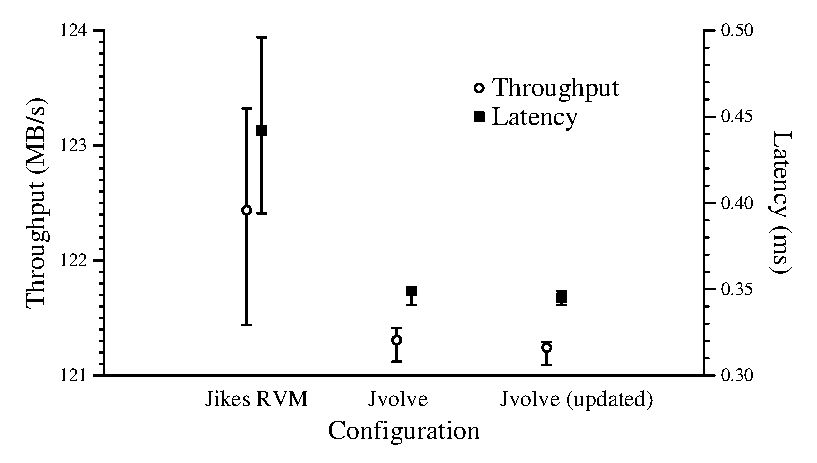
\includegraphics{graphs/jetty-throughput-latency}}
\caption{Throughput and latency measurements of Jetty webserver v5.1.6\label{fig:jetty}}
\end{center}
\end{figure}

% \begin{figure}[t]
\begin{center}
\scalebox{0.63}{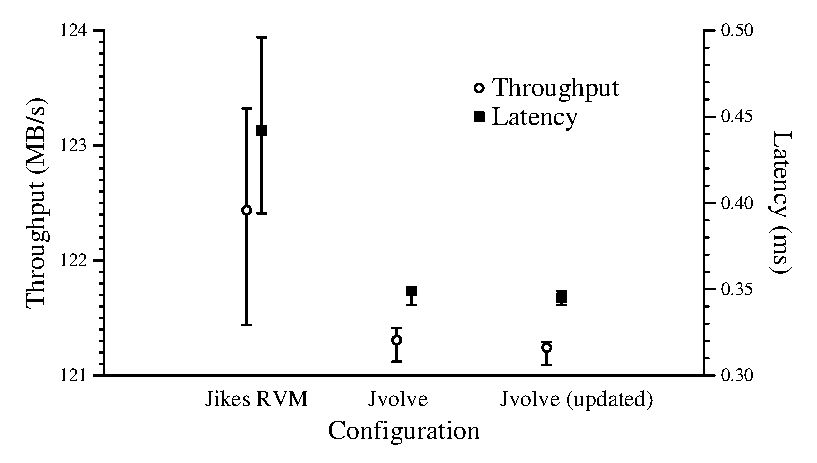
\includegraphics{graphs/jetty-throughput-latency}}
\caption{Throughput and latency measurements of Jetty webserver v5.1.6\label{fig:jetty}}
\end{center}
\end{figure}

% \begin{table*}[t]
\begin{footnotesize}
\begin{center}
\begin{tabular}{|r|r|rrrrrrrrrrr|}
                                                                                                                                   \hline
\multirow{2}{*}{\# objects}     & \multicolumn{1}{c}{Heap}   & \multicolumn{11}{|c|}{Fraction of updated objects \T}            \\
                                & \multicolumn{1}{c|}{size}  &
                       0\%  &   10\%  &   20\%  &   30\%  &   40\%  &   50\%  &   60\%  &   70\%  &   80\%  &   90\%  &  100\%  \\ \hline
\multicolumn{13}{|c|}{Garbage collection time (ms) \T}                                                                          \\ \hline \T
 280000 &  160 MB &    78.2 &    81.3 &    83.1 &    89.3 &    99.0 &   103.2 &   108.3 &   113.2 &   113.3 &   120.3 &   120.0 \\
 770000 &  320 MB &   148.9 &   165.0 &   181.9 &   195.8 &   213.2 &   223.2 &   237.0 &   249.0 &   262.0 &   269.5 &   278.6 \\
1760000 &  640 MB &   313.3 &   347.7 &   382.9 &   416.0 &   449.8 &   478.9 &   506.8 &   534.0 &   558.8 &   583.7 &   601.5 \\
3670000 & 1280 MB &   615.4 &   694.6 &   763.0 &   833.6 &   900.1 &   965.9 &  1019.0 &  1076.4 &  1129.9 &  1181.2 &  1217.5 \\ \hline
\multicolumn{13}{|c|}{Running transformation functions (ms) \T}                                                                 \\ \hline \T
 280000 &  160 MB &     0.1 &    13.0 &    23.2 &    34.6 &    43.9 &    54.0 &    62.7 &    74.5 &    84.1 &    93.9 &   104.2 \\
 770000 &  320 MB &     0.1 &    33.7 &    63.1 &    91.2 &   116.8 &   145.4 &   173.9 &   201.0 &   231.3 &   262.0 &   292.6 \\
1760000 &  640 MB &     0.1 &    77.9 &   143.9 &   207.7 &   269.5 &   333.7 &   397.6 &   464.0 &   534.6 &   604.5 &   674.9 \\
3670000 & 1280 MB &     0.1 &   160.8 &   299.2 &   429.4 &   560.2 &   693.8 &   827.3 &   975.0 &  1119.6 &  1263.7 &  1405.4 \\ \hline
\multicolumn{13}{|c|}{Total DSU pause time (ms) \T}                                                                             \\ \hline \T
 280000 &  160 MB &    82.8 &    99.0 &   109.5 &   128.0 &   147.6 &   161.2 &   174.5 &   192.8 &   202.5 &   218.8 &   228.1 \\
 770000 &  320 MB &   153.6 &   202.9 &   249.0 &   291.4 &   334.5 &   372.6 &   414.8 &   455.4 &   498.1 &   535.3 &   576.8 \\
1760000 &  640 MB &   316.6 &   429.5 &   530.5 &   627.2 &   723.4 &   816.0 &   908.6 &  1002.6 &  1097.5 &  1191.5 &  1281.2 \\
3670000 & 1280 MB &   618.7 &   859.0 &  1065.9 &  1269.9 &  1466.1 &  1663.6 &  1850.8 &  2054.2 &  2253.1 &  2448.5 &  2627.9 \\ \hline
\end{tabular}
\end{center}
\end{footnotesize}
\caption{Microbenchmark results: \DSU{} update pause time (in ms) for various heap sizes}
\label{tab:microbench}
\end{table*}


\paragraph{Jetty performance.}
To see the effect of updating on application performance, we measured Jetty
under various configurations using httperf, a webserver
benchmarking tool.\footnote{\url{http://www.hpl.hp.com/research/linux/httperf}}  We used httperf to issue roughly 800 new connection
requests/second, which we observed to be Jetty's saturation rate.
Each connection makes 5 serial requests for a 40 Kbyte file. Httperf
reports average throughput and average per-request latency over a 60 second period. We
ran this experiment 21 times and report the median and
quartiles of the throughput and latency reports. With 21 runs, the range between
the quartiles serves as a 98\% confidence interval~\cite{PrattGibbons81}.
In order to eliminate network traffic
effects, we ran the server on two cores of a quad-core machine and the
client on another core.

Figure~\ref{fig:jetty} shows our results in tabular form and plotted graphically.  The second and third columns
of the table
report the median throughput and the range between the two quartiles.
The third column and fourth column report the median latency and the
inter-quartile range.  The
first and seconds rows illustrate the performance of Jetty version 5.1.6
running on stock \JikesRVM{} and \DSU, respectively. The third row shows
the performance on \DSU{} of Jetty 5.1.6 dynamically updated from version
5.1.5 prior to the start of the experiment.
% \todo{Find a way to introduce the graph} Figure~\ref{fig:jetty} plots the results shown in the table.
The performance of the two \DSU{} configurations
is essentially identical: the two configurations' corresponding
inter-quartile ranges largely overlap.
The performance of \DSU{} is also quite similar to the performance of
stock \JikesRVM.  There are many small differences between \DSU{} and the stock
implementation that change VM code size, code layout, and garbage
collection behavior.  These differences may impact performance
directly and they may indirectly affect other elements of the VM,
such as the timing of garbage collections and JIT
optimizations (such indirect effects make VMs notoriously difficult to
benchmark~\cite{dacapo-cacm}).


%%% Local Variables: 
%%% mode: latex
%%% TeX-master: "../pldi64"
%%% End: 

% \begin{table*}[t]
\begin{footnotesize}
\begin{center}
\begin{tabular}{|r|r|rrrrrrrrrrr|}
                                                                                                                                   \hline
\multirow{2}{*}{\# objects}     & \multicolumn{1}{c}{Heap}   & \multicolumn{11}{|c|}{Fraction of updated objects \T}            \\
                                & \multicolumn{1}{c|}{size}  &
                       0\%  &   10\%  &   20\%  &   30\%  &   40\%  &   50\%  &   60\%  &   70\%  &   80\%  &   90\%  &  100\%  \\ \hline
\multicolumn{13}{|c|}{Garbage collection time (ms) \T}                                                                          \\ \hline \T
 280000 &  160 MB &    78.2 &    81.3 &    83.1 &    89.3 &    99.0 &   103.2 &   108.3 &   113.2 &   113.3 &   120.3 &   120.0 \\
 770000 &  320 MB &   148.9 &   165.0 &   181.9 &   195.8 &   213.2 &   223.2 &   237.0 &   249.0 &   262.0 &   269.5 &   278.6 \\
1760000 &  640 MB &   313.3 &   347.7 &   382.9 &   416.0 &   449.8 &   478.9 &   506.8 &   534.0 &   558.8 &   583.7 &   601.5 \\
3670000 & 1280 MB &   615.4 &   694.6 &   763.0 &   833.6 &   900.1 &   965.9 &  1019.0 &  1076.4 &  1129.9 &  1181.2 &  1217.5 \\ \hline
\multicolumn{13}{|c|}{Running transformation functions (ms) \T}                                                                 \\ \hline \T
 280000 &  160 MB &     0.1 &    13.0 &    23.2 &    34.6 &    43.9 &    54.0 &    62.7 &    74.5 &    84.1 &    93.9 &   104.2 \\
 770000 &  320 MB &     0.1 &    33.7 &    63.1 &    91.2 &   116.8 &   145.4 &   173.9 &   201.0 &   231.3 &   262.0 &   292.6 \\
1760000 &  640 MB &     0.1 &    77.9 &   143.9 &   207.7 &   269.5 &   333.7 &   397.6 &   464.0 &   534.6 &   604.5 &   674.9 \\
3670000 & 1280 MB &     0.1 &   160.8 &   299.2 &   429.4 &   560.2 &   693.8 &   827.3 &   975.0 &  1119.6 &  1263.7 &  1405.4 \\ \hline
\multicolumn{13}{|c|}{Total DSU pause time (ms) \T}                                                                             \\ \hline \T
 280000 &  160 MB &    82.8 &    99.0 &   109.5 &   128.0 &   147.6 &   161.2 &   174.5 &   192.8 &   202.5 &   218.8 &   228.1 \\
 770000 &  320 MB &   153.6 &   202.9 &   249.0 &   291.4 &   334.5 &   372.6 &   414.8 &   455.4 &   498.1 &   535.3 &   576.8 \\
1760000 &  640 MB &   316.6 &   429.5 &   530.5 &   627.2 &   723.4 &   816.0 &   908.6 &  1002.6 &  1097.5 &  1191.5 &  1281.2 \\
3670000 & 1280 MB &   618.7 &   859.0 &  1065.9 &  1269.9 &  1466.1 &  1663.6 &  1850.8 &  2054.2 &  2253.1 &  2448.5 &  2627.9 \\ \hline
\end{tabular}
\end{center}
\end{footnotesize}
\caption{Microbenchmark results: \DSU{} update pause time (in ms) for various heap sizes}
\label{tab:microbench}
\end{table*}

\begin{figure}[t]
\begin{center}
\scalebox{0.69}{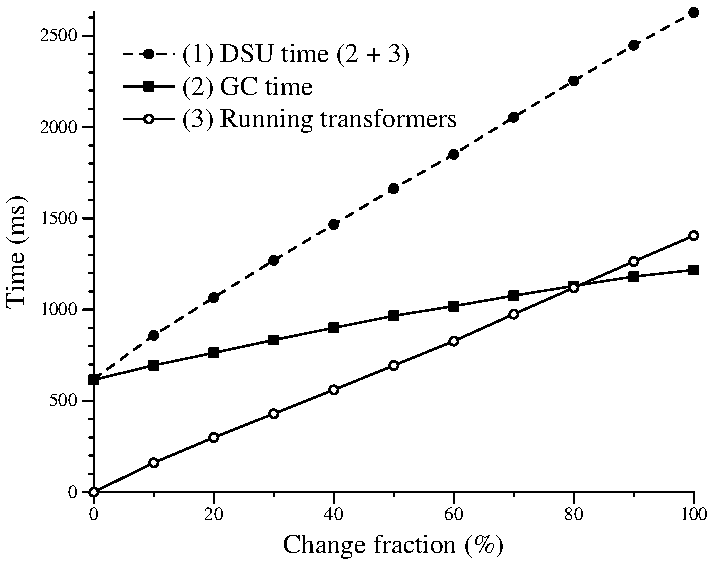
\includegraphics{graphs/microbench}}
\caption{Microbenchmark pause times with a heap size of 1280 MB containing
3.67 million objects\label{fig:microbench}}
\end{center}
\end{figure}


\paragraph{Microbenchmarks.}
The two dominant factors that determine \DSU{} update time are the time to
perform a GC, determined by the number of objects, and the time to run
object transformers, determined by the fraction of objects being
updated.  To measure the cost of each, we devised a simple 
microbenchmark that creates an array of objects and transforms a specified
fraction of these objects when a \DSU{} update is triggered. The
microbenchmark has two simple classes, \texttt{Change} and
\texttt{NoChange}. Both contain three integer fields, and three reference
fields that are always {\tt null}. The update adds an integer field to
{\tt Change}. The user-provided object transformation function copies the
existing fields and initializes the new field to zero.
% The benchmark contains two arrays,
% one for \texttt{Change} objects and one for \texttt{NoChange} objects.
We measure the cost of performing an update while varying the total
number of objects and the fraction of objects of each type. The number of
objects is the maximum that can fit in heap sizes 32, 64, 128 and 256
MB.  Note that \JikesRVM{}'s heap includes VM data structures as well. We
measure the running time in a generous heap, five times the minimum required size, such that the only collections are those DSU triggers. We report the
median of 21 runs.

Table~\ref{tab:microbench} shows the elapsed time
while varying the number of total objects and the fraction of the objects that are updated.  The
variance was insignificant, so we do not report it.   % KSM: I deleted the first row, since it is the only one with this problem, which is due to other costs dominating, e.g., stack walking etc. because apparently copying 40,000 objects takes no time at all. \todo{some of the
%   results are unintuitive; e.g., the time goes down as you move to the
%   right, sometimes.  Make a comment here about that being the way of
%   things with sophisticated machines?  Can't blame it on the
%   variance.}
The first group of rows reports
garbage collection time, the second group reports the time to transform
all updated objects, and the final group reports the total update time, which
includes the sum of the GC and transformation time, the time to load and install the updated classes, synchronize
running threads, and find a DSU safe point. 
The first column of the table shows the number of objects in the test, and
the second column the heap size. Columns 3 though 13 show pause times for
varying fractions (from 0\% to 100\%) of updated objects. 
% Looking at
% the last column of the table, we can see that the GC time results
% (first group of rows) for
% various heap sizes are roughly the same as the transformation time
% results (second group of rows), showing the time to transform an
% object to be roughly equal to the time to copy an object in the collector.

To shed light on the results in the table,
Figure~\ref{fig:microbench} plots collection time, transformer time and
total update time for the microbenchmark with 3.67 million objects in a
1280 MB heap.  The figure shows that the costs of garbage collection and
transformation increase  as a function of the number of changed objects.  The slope of the ``GC time'' line illustrates the cost to deal
with an increasing number of transformed objects.  This cost includes
creating an additional copy of each transformed object; creating the
update log entry with a pointer to the old and new copy; and caching a
pointer to the old copy from the new copy.  The slope of the
``Running transformers'' line illustrates the added cost of iterating
over the update log and actually running the transformers.  This extra
processing to handle transforming objects increases the total pause
time with all objects updated by roughly four times compared to the
pause time with no object updated.  The ``Running
Transformers'' line is steeper than the ``GC time'' line, revealing that
the cost of running transformers is higher than the extra copying cost
incurred during GC\@.

Transformations are more expensive than standard copying GC. The GC uses
\texttt{memcopy}, which is highly optimized, whereas our transformer
functions use reflection to look up \texttt{jvolveObject}, and this
function copies one field at a time.  One optimization would be to eliminate the log by copying
the old and new objects to their own space and % appending to each one a
% pointer to their corresponding new object.
walking through and transforming each object.
The cost of reflection could be
reduced by caching the lookup, but even then a na\"ively compiled
field-by-field copy is much slower than the collector's
highly-optimized copying loop.  % Another possible optimization is to
% specially compile transformers to replace idiomatic use of copying
% assignments to contiguous fields by a \texttt{memcopy} over the
% corresponding range.


%%% Local Variables: 
%%% mode: latex
%%% TeX-master: "../pldi64"
%%% End: 



\newcommand{\ChangedClassesColumn}{third}
\begin{table}
\begin{footnotesize}
\begin{center}
\begin{tabular}{|l||c||c|c|c|r|c|c|} \hline \T
Ver.    & \#      & \multicolumn{6}{c|}{\# changed} \\
        & classes & \multicolumn{1}{c|}{classes} & \multicolumn{3}{c|}{methods} & \multicolumn{2}{c|}{fields} \\
        & added   &         & add & del & \multicolumn{1}{c|}{chg}             & add & del \\ \hline \hline \T
5.1.1   & 0       & 14      &\ 4  & 1   &  38/0            &  0  & 0   \\
5.1.2   & 1       &\ 5      &\ 0  & 0   &  12/1            &  0  & 0   \\
5.1.3*  & 3       & 15      & 19  & 2   &  59/0            & 10  & 1   \\
5.1.4   & 0       &\ 6      &\ 0  & 4   &   9/6            &  0  & 2   \\
5.1.5   & 0       & 54      & 21  & 4   & 112/8            &  5  & 0   \\
5.1.6   & 0       &\ 4      &\ 0  & 0   &  20/0            &  5  & 6   \\
5.1.7   & 0       &\ 7      &\ 8  & 0   &  11/2            &  9  & 3   \\
5.1.8   & 0       &\ 1      &\ 0  & 0   &   1/0            &  0  & 0   \\
5.1.9   & 0       &\ 1      &\ 0  & 0   &   1/0            &  0  & 0   \\
5.1.10  & 0       &\ 4      &\ 0  & 0   &   4/0            &  0  & 0   \\ \hline
\end{tabular}
\end{center}
\end{footnotesize}
\caption{Summary of updates to Jetty}
\label{tab:jetty-changes}
\end{table}

\subsection{Jetty webserver}
\label{subsec:jetty}

Jetty is a popular webserver written in Java. It supports static
and dynamic content and can be embedded 
within other Java applications. \JikesRVM, and thus \DSU, is not able to run the
most recent versions of Jetty (6.x).  Therefore we considered 11
versions, consisting of 5.1.0 through 5.1.10 (the last version prior to
version 6).  Version 5.1.10 contains 317 classes and about 45,000 lines
of code.  Table~\ref{tab:jetty-changes} shows a summary of the changes
in each update.  Each row tabulates the changes relative
to the prior version. For the column listing changed methods, the
notation $x/y$ indicates that $x+y$ methods were changed, where $x$
changed in body only, and $y$ changed their type signature as well.
For dynamic updating systems that only support changes to method
bodies, only the first and last three of the ten updates could be
supported, since the rest either change method signatures
and/or add or delete fields.

\paragraph{Reaching a safe point in Jetty.}
We  successfully wrote dynamic updates to all
versions of Jetty that we examined. For each version starting at 5.1.0, we ran
Jetty under full load. After 30 seconds we tried to apply the update to the
next version. We did this five times per version.  Other than the
update to 5.1.3, all versions immediately 
reached a safe point every time, with no need of return barriers.

We could not apply the update to version 5.1.3 (denoted with an
asterisk in the table) 
because \DSU{} was never able to reach a safe point. The update modified
{\tt ThreadedServer.accept\-Socket()}, a method that waits for a connection
from the client, and this method is nearly always on stack. 
We installed a return barrier that is triggered when {\tt
  acceptSocket} returns, but this barrier is not sufficient to perform the
update since the main methods of several threads were themselves
modified. For example, we also install a return barrier on {\tt
  Pool\-Thread.run()}, but this barrier is never triggered because
this method never becomes inactive.

% REFACTOR: add para back if we get things to work.
% We refactored the various long-running main methods in versions 5.1.2 and
% 5.1.3 to extract the modified bodies of long running methods into separate
% methods and leave the main method containing the loop unmodified between
% the two versions.  (This sort of transformation is performed by other
% systems automatically by programmer directive in
% Ginseng~\cite{neamtiu06dsu}.) 
% When we attempted to perform a dynamic update, \DSU{}
% installed a return barrier for {\tt acceptSocket()}. This function waits
% for a connection and returns after a timeout. \DSU{} was able to update the
% application when this function returned. 

% To understand why, we instrumented the VM to emit information about
% restricted method set and, if a safe point cannot be reached, which
% restricted method was active. 

% \suriya{The following information about inlining is commented out. What
% should we do with this? See .tex file}
%     For each version, starting at 5.1.0, we
%     ran Jetty under full load.  After 30 seconds we tried to apply the
%     update to the next version; if a safe point could not be immediately
%     reached, we deemed the attempt as failed.
%     The results are presented in
%     Table~\ref{tab:inlining}.  Column 2 shows the number of times out of
%     five such runs where the application reached a safe point.  The methods
%     whose presence on a thread stack precluded the application from
%     reaching a safe point are mentioned below the table.  For the update to
%     5.1.3, the offending method was always active because it contained an
%     infinite loop.  The other updates either always succeeded, or did after a
%     small number of retries.
%     
%     Column 3 contains the total number
%     of methods in the program at runtime, where the number in parentheses is the
%     number of those which the compiler inlined when using aggressive
%     optimization.
%     This provides an upper bound on the effect of inlining in reaching a
%     safe point.  The next group of columns contains the restricted method
%     set. Each column in the group specifies the number of methods loaded at
%     run time by the VM, followed by the total number of methods in that
%     category in the program. The first column in this group is the number of methods in
%     classes involved in a class update. Recall that when a class is updated, say by adding
%     a field, all its methods are considered restricted (see section~\ref{sec:safe}).
%     \suriya{Provide reference to where we explain restricted. and redefine
%     restricted}
%     The second column in this group is the number of methods whose
%     bodies are updated, the third is the number of methods
%     indirectly updated, and the fourth sums these, with the number of methods
%     that were inlined written in parentheses. % The first and second
%     % columns in this group together constitute all the methods of classes that
%     % were changed, as enumerated in the \ChangedClassesColumn{} column in table~\ref{tab:jetty-changes}.
%     The final two columns list
%     the total number of methods in the restricted set; they differ from the
%     first number in the fourth column by the number of (transitively)
%     inlined callers of the restricted methods that were not already
%     restricted.  The final column uses \DSU{}'s OSR analysis to determine the
%     number of restricted methods although OSR itself was not applied.
%     
%     The table shows that both indirect method calls \suriya{or updates?} and inlining significantly
%     add to the size of the restricted set.  Inlining though, is small by
%     comparison, because all callers of an updated class's methods are
%     \emph{already} included in the indirect set. Therefore, inlining these
%     methods adds no further restriction.
%     In most cases OSR support would dramatically reduce the number of
%     restricted methods and increase the likelihood of reaching a DSU safe
%     point.
%     Interestingly, having a greater number of restricted methods overall
%     does not necessarily reduce the likelihood that an update will take
%     effect; rather, it depends on the frequency with which methods in this
%     set are on the stack.

%%% Local Variables: 
%%% mode: latex
%%% TeX-master: "../pldi64"
%%% End: 

\subsection{JavaEmailServer}
\label{subsec:jes}

\begin{table}[t]
\begin{footnotesize}
\begin{center}
\begin{tabular}{|l||c|c||c|r|c|r|r|c|} \hline \T
Ver.   & \multicolumn{2}{c||}{\# classes} &    \multicolumn{6}{c|}{\# changed} \\
       & add & del & classes & \multicolumn{3}{c|}{methods} & \multicolumn{2}{c|}{fields} \\
       &     &     &         & add & del & chg   & add & del \\ \hline \hline \T
1.2.2  & 0   & 0   & 3       & 0   & 0   & 3/0   & 0   & 0   \\
1.2.3  & 0   & 0   & 7       & 0   & 0   & 14/2  & 12  & 0   \\
1.2.4  & 0   & 0   & 2       & 0   & 0   & 4/0   & 0   & 0   \\
1.3*   & 4   & 9   & 2       & 11  & 3   & 6/9   & 12  & 5   \\
1.3.1  & 0   & 0   & 2       & 0   & 0   & 4/0   & 0   & 0   \\
1.3.2  & 0   & 0   & 8       & 4   & 2   & 4/2   & 3   & 1   \\
1.3.3  & 0   & 0   & 4       & 0   & 0   & 3/0   & 0   & 0   \\
1.3.4  & 0   & 0   & 6       & 2   & 0   & 6/0   & 2   & 0   \\
1.4    & 0   & 0   & 7       & 6   & 1   & 4/1   & 6   & 0   \\ \hline
\end{tabular}
\end{center}
\end{footnotesize}
\caption{Summary of updates to JavaEmailServer}
\label{tab:jes-changes}
\end{table}

For JavaEmailServer, we considered 10 versions---1.2.1 through
1.4---spanning a duration of about two years.   Version 1.4 
consists of 20 classes and about 5000 lines of code. 
Table~\ref{tab:jes-changes} shows the summary of changes for each new
version. Approaches that only support updates to method bodies will be able
to handle only four of these updates. We
could successfully construct updates for all versions we examined, and
we could successfully apply all of them except the update to version 1.3.
This update reworks the configuration framework of the server, among other
things removing a GUI tool for user administration and adding several
new classes that implement a file-based configuration system.  As a result, many of
the classes are modified to point to a new configuration object.
Among these classes are threads with infinite processing loops (e.g., to accept
POP and SMTP requests). Because these threads are always active, the
safety condition can never be met and thus the update cannot be
applied.

The update from 1.3.1 to 1.3.2 indirectly changes the
\texttt{SMTP\-Sen\-d\-er.run()} and \texttt{Pop3\-Processor.run()} methods.  These
methods contain processing loops run by several threads.  Though these
methods are always running, \DSU{} applies OSR and the update succeeds.
\DSU{} also uses OSR for the update from 1.3.2 to 1.3.3.
%MWH: suriya says this statement just isn't true.  Updates fine.
% A method used to process connections was also changed, and this method
% is frequently active when the server is under load.  (A similar
% method was changed in the update to version 1.3.3.)  A return barrier
% installed on this method permits the update to take effect.  

\begin{table}[t]
\begin{footnotesize}
\begin{center}
\begin{tabular}{|l||c|c||c|c|c|r|c|c|} \hline \T
Ver.   & \multicolumn{2}{c||}{\# classes} &    \multicolumn{6}{c|}{\# changed}             \\
       & add & del & classes & \multicolumn{3}{c|}{methods} & \multicolumn{2}{c|}{fields}  \\
       &     &     &         & add & del & chg   & add & del                               \\ \hline \hline \T
1.06   & 4   & 1   & 1       & 0   & 0   & 3/0   & 1   & 0                                 \\
1.07   & 0   & 0   & 3       & 4   & 0   & 14/0  & 5   & 0                                 \\
1.08   & 0   & 1   & 3       & 2   & 0   & 10/0  & 0   & 2                                 \\ \hline
\end{tabular}
\end{center}
\end{footnotesize}
\caption{Summary of updates to CrossFTP server}
\label{tab:crossftp-changes}
\end{table}

\subsection{CrossFTP server}
\label{subsec:crossftp}
CrossFTP server is an easily configurable, security-enabled FTP server.
CrossFTP allows simple configuration through a GUI and more advanced
customization using configuration files. We did not use the GUI interface
and therefore do not consider changes to that part of the program.  We
looked at 4 versions--- 1.05 through 1.08, details shown in Table~\ref{tab:crossftp-changes}---spanning a duration of more
than a year. Version 1.08 contains about 18,000 lines of code spread across
161 classes. \DSU{} successfully applies all three updates to this
application.  Note that since all updates either add or delete fields,
simple method body updating support on its own would be insufficient.

\DSU{} could only apply the update from version 1.07 to 1.08 when the
server was relatively idle.
%MWH: I added relatively here, since the update should work when there
%is one connection, by our explanation: i.e., one thread running
%RequestHandler.run() will hit its return barrier and the update takes
%place.  Maybe two connections too, if you get lucky, etc.
The server runs a new {\tt RequestHandler} thread to process each FTP
session, and the \texttt{RequestHandler.run()} method was changed by
the update.   \DSU{} installs a return barrier on this method,
but with many active sessions, this method is essentially always on stack,
preventing the update.  Future work could address this problem using scheduler support
for coordinating updates among active threads~\cite{neamtiu09stump}.

